\documentclass[spanish, a4paper, 12pt, twoside, openany,final]{book} 
\usepackage{textcomp}
\usepackage[T1]{fontenc, url}
\usepackage[utf8]{inputenc}
\usepackage{titlesec}
\setcounter{secnumdepth}{4}
\usepackage{multirow}      
\usepackage{algpseudocode} 
\usepackage{multicol}
\usepackage[Algoritmo]{algorithm}               
\usepackage{minted}                             
\usepackage{adjustbox}                          
\usepackage{graphicx}                           
\usepackage{amsmath, amssymb, amsthm}           
\usepackage{parskip}                            
\urlstyle{sf}                                   
\usepackage{color}                              
\usepackage{subcaption}                         
\usepackage[toc,page]{appendix}                 
\usepackage{chngcntr}                           
\counterwithin{table}{section}                  
\counterwithin{figure}{section}                 
\numberwithin{equation}{section}                
\hyphenpenalty=100000                           
\sloppy                                         
\raggedbottom                                   
\usepackage{xparse,nameref}                     
\usepackage[bottom,hang,flushmargin]{footmisc}  
\interfootnotelinepenalty=10000                 
\usepackage{lipsum}                     

% --------- Editar de aquí en adelante --------

% ----- Apariencia e idioma ----- 
\usepackage[spanish]{babel}                                         % Idioma
\graphicspath{{Images/}{../Images/}}                                % Dónde estarán las imágenes
\usepackage[left=4cm,top=4cm,bottom=2.5cm,right=2.5cm]{geometry}    % Márgenes del documento
\usepackage{setspace}                                               % Permite elegir el interlineado
\linespread{1.3}                                                    % Interlineado de uno y medio. 1.6 es interlineado doble.
\usepackage{microtype}                                              % Permite la modificación de los caracteres.


% ----- Secciones ----- % ESTA PARTE SE UTILIZA EN CASO DE USAR LA CLASE ARTICLE

% \titleformat*{\section}{\LARGE\bfseries}                  % Forma del título de \section 
% \titleformat*{\subsection}{\Large\bfseries}               % Forma del  título de \subsection
% \titleformat*{\subsubsection}{\large\bfseries}            % Forma del  título de \subsubsection 

% Las siguientes tres líneas crean el comando \paragraph con la forma del título correcta.

% \titleformat{\paragraph} 
% {\normalfont\normalsize\bfseries}{\theparagraph}{1em}{}
% \titlespacing*{\paragraph}
% {0pt}{3.25ex plus 1ex minus .2ex}{1.5ex plus .2ex}
%-----------------------------------------------

% ----- Figuras y tablas ----- 
\usepackage{fancyhdr}                           % Permite formatear las cabeceras, pies, enumeración, etc.
\usepackage{subfiles}                           % Para agregar los capítulos que se escriben aparte.
\usepackage{array}                              % Para ordenar texto y ecuaciones.
\usepackage[rightcaption]{sidecap}              % Permite agregar texto lateral
\usepackage{wrapfig}                            % Permite poner figuras con texto al rededor.
\usepackage{float}                              % Permite poner figuras en cualquier lugar.
\usepackage[labelfont=bf]{caption}              % Texto en negrita para descripciones (\caption)
\usepackage{amsmath}
\usepackage{amssymb}
\usepackage[para]{threeparttable}               % Tablas vistosas, mirar antes de utilizar.
\usepackage{url}                                % Permite el uso de enlaces URL.
\usepackage[table,xcdraw,dvipsnames]{xcolor}    % Agranda la cantidad de colores.
\usepackage{makecell}                           % Ayuda en la creación de tablas
\usepackage{hhline}                             % Agranda las opciones de las líneas
\usepackage{textcomp}                           % Símbolo de derechos de autor


% ----- Referencias -----
\usepackage{natbib}                                                     % Ambiente de referencias utilizado.
\bibliographystyle{apalike}                                                 % Estilo de referencias APA.
\def\biblio{\clearpage\bibliographystyle{apalike}\bibliography{References}} % Define el comando \biblio para referencias en subarchivos- NO CAMBIAR


% ----- Cabecera y pies -----
\pagestyle{fancy}                           % Se define el estilo fancy
\fancyhead[RO,LE]{\thepage}                 % Número de página en la izquierda para par y derecha para impar
\fancyhead[RE,LO]{\nouppercase{\rightmark}} % Nombre del capítulo en la derecha para par y la izquierda para impar en la cabecera
%\renewcommand{\headrulewidth}{0pt}         % Cambiar para línea más gruesa
\fancyfoot{}                                % Saca el número de la página abajo.

\fancypagestyle{plain}{                     % Se redefine el estilo automático (plain) para que calce con el resto. En particular la 1ra página de cada capítulo
\fancyhf{}                                  % Elimina la cabecera y los pies
\fancyhead[RO,LE]{\thepage}                 % Número de página en la izquierda para par y derecha para impar
\fancyhead[RE,LO]{\nouppercase{\leftmark}}  % Nombre del capítulo en la derecha para par y la izquierda para impar en la cabecera
%\renewcommand{\headrulewidth}{0pt}         % Cambiar para línea más gruesa
\fancyfoot{}                                % Elimina el número de la página abajo
}

%------------------- Cabecera del Resumen y Agradecimientos--------------

\fancypagestyle{resumen}{                   % Se redefine el estilo resumen para que calce con el resto. 
\fancyhf{}                                  % Elimina la cabecera y los pies
\fancyhead[RO,LE]{\thepage}                 % Número de página en la izquierda para par y derecha para impar
\fancyhead[RE,LO]{\nouppercase{Resumen}}    % Nombre del capítulo en la derecha para par y la izquierda para impar en la cabecera
%\renewcommand{\headrulewidth}{0pt}         % Cambiar para línea más gruesa
\fancyfoot{}                                % Elimina el número de la página abajo
}

\fancypagestyle{abstract}{                  % Se redefine el estilo resumen para que calce con el resto. 
\fancyhf{}                                  % Elimina la cabecera y los pies
\fancyhead[RO,LE]{\thepage}                 % Número de página en la izquierda para par y derecha para impar
\fancyhead[RE,LO]{\nouppercase{Abstract}}   % Nombre del capítulo en la derecha para par y la izquierda para impar en la cabecera
%\renewcommand{\headrulewidth}{0pt}         % Cambiar para línea más gruesa
\fancyfoot{}                                % Elimina el número de la página abajo
}

\fancypagestyle{agradecimientos}{                   % Se redefine el estilo resumen para que calce con el resto. 
\fancyhf{}                                          % Elimina la cabecera y los pies
\fancyhead[RO,LE]{\thepage}                         % Número de página en la izquierda para par y derecha para impar
\fancyhead[RE,LO]{\nouppercase{Agradecimientos}}    % Nombre del capítulo en la derecha para par y la izquierda para impar en la cabecera
%\renewcommand{\headrulewidth}{0pt}                 % Cambiar para línea más gruesa
\fancyfoot{}                                        % Elimina el número de la página abajo
}

% ----- Cabecera de la portada ----- 
\fancypagestyle{frontpage}{             % Se define el estilo frontpage.
	\fancyhf{}                          % Elimina la cabecera y los pies
	\renewcommand{\headrulewidth}{0pt}  % Elimina líneas en cabecera
	\renewcommand{\footrulewidth}{0pt}  % Elimina líneas en pies
	\vspace*{1\baselineskip}
	
 \fancyhead[L]{ 
\includegraphics[width=0.7in]{escudo_udec.png}\hspace{2cm}}
	\fancyhead[C]{UNIVERSIDAD DE CONCEPCIÓN
	\linebreak FACULTAD DE INGENIERÍA
    \linebreak DEPARTAMENTO DE INGENIERÍA CIVIL INDUSTRIAL}
    \fancyhead[R]{\hspace{1cm}
\includegraphics[width=0.7in]{Images/FI_Udec.png}}
	
}

% ----- Enlaces clickeables --------
\usepackage{hyperref}   % Permite que todo el documento sea clickeable.
\newcommand\myshade{85} % Permite la redefinición de colores a gusto del usuario

% Para elegir colores propios mirar los nombres relacionados con dvipsnames, aquí un url con los nombres de dvipsnames: https://www.overleaf.com/learn/latex/Using_colours_in_LaTeX

\colorlet{mylinkcolor}{DarkOrchid}   %Hiperlinks internos
\colorlet{mycitecolor}{YellowOrange} %Citas
\colorlet{myurlcolor}{Aquamarine}    %Urls

% Para dejar el documento sin texto en colores cambiar las tres líneas anteriores a Black.

\hypersetup{  %Define la forma en que se verán las cosas clickeables.
  	linkcolor  = mylinkcolor!\myshade!black,    % Aplica el color definido arriba. En este caso DarkOrchid
  	citecolor  = mycitecolor!\myshade!black,    % Aplica el color definido arriba. En este caso YellowOrange
  	urlcolor   = myurlcolor!\myshade!black,     % Aplica el color definido arriba. En este caso Aquamarine
  	colorlinks = true,                          % Elimina las cajas al rededor de lo clickeable y lo reemplaza por palabras a color.
}


%--------------------------------------------------------------------------------------------------------------------------
% ------------------------------------------ Aquí empieza el documento ----------------------------------------------------
%--------------------------------------------------------------------------------------------------------------------------

\usepackage{tikz}
\begin{document}
\def\biblio{}   % Resetea el comando biblio, de lo contrario una lista de referencias será producida después de cada capítulo
                % resets the biblio command, if not here a new reference list will be produced after every chapter

\begin{titlepage}
	
	\newgeometry{top=1 in, bottom=1 in, left=1 in, right= 1 in} 
	
	\thispagestyle{frontpage}
	
	\begin{center}
		
		\vspace*{4\baselineskip}
		
		
		{\Huge \textbf{UN ALGORITMO BASADO EN MACHINE LEARNING PARA EL PROBLEMA POLINOMIAL ROBUSTO DE LA MOCHILA\\}}
		\vspace*{1.5\baselineskip}
		
		%\large{\textit{subtítulo}}\\
		
		\vspace*{1,5\baselineskip}
		
		\large{\textbf{Por: José Ignacio González Cortés}}\\
		
		\vspace{1,5\baselineskip}
		
		\large{Memoria de titulo presentada a la Facultad de ingeniería de la Universidad de Concepción para optar al título profesional de ingeniero civil industrial} 
		
		\vspace{1,5\baselineskip}
		Octubre 2023\\ %Mes y año de la tesis, solo primera letra del mes en mayúsculas
		Concepción, Chile %Ciudad y país de publicación.
		\vspace{1,5\baselineskip}
		
		\large{\textbf{Profesor Guía: Carlos Contreras Bolton}}\\
		
	\end{center}
	
	\vspace*{4\baselineskip}
	
\end{titlepage}


\vfill

%\begin{center}
%\begin{figure}
%    \centering
%    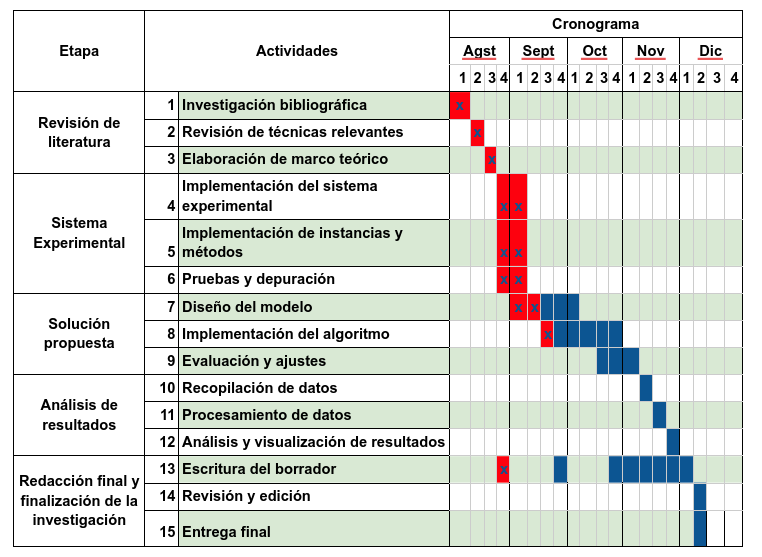
\includegraphics[width=1.1\linewidth]{Images/image.png}
%    \caption{Cronograma actual}
%    \label{fig:cronograma}
%\end{figure}
%\end{center}

%----------------Página de derechos de autor: elegir entre a) o b) y borrar/comentar la opción NO utilizada-----------------
\thispagestyle{empty}
\mbox{}                         % Ayuda a bajar el texto
\vfill                          % Deja el texto al fondo
\textcopyright\ 2023, José Ignacio González Cortés \\ % Derechos de autor
%a)
Ninguna parte de esta memoria puede reproducirse o transmitirse bajo ninguna forma o por ningún medio o procedimiento, sin permiso por escrito del autor.\\\\
%b)
Se autoriza la reproducción total o parcial, con fines académicos, por cualquier medio o procedimiento, incluyendo la cita bibliográfica del documento
\vspace{1cm}    % lo separa del fondo
\restoregeometry % Devuelve los márgenes después de la portada


%----------------Página de calificaciones (opcional), descomentar para generar-----------------

% Editar en Otros -> Calificaciones.tex

%%Las calificaciones entregan la misma información de la portada y se le agrega la nota y la firma. Esta página es opcional.
\begin{titlepage}
	
	\newgeometry{top=1 in, bottom=1 in, left=1 in, right= 1 in} 
	
	\thispagestyle{frontpage}
	
	\begin{center}
		
		\vspace*{4\baselineskip}
	
		
		{\Huge \textbf{TÍTULO PRINCIPAL\\}}%No abreviar, no subrayar, no usar comillas. Se escribe completamente en mayúsculas
		        \vspace*{1.5\baselineskip}

		\large{\textit{subtítulo}}\\ %No abreviar, no subrayar, no usar comillas. Solo la priemra letra usa mayúsculas
		
        \vspace*{1,5\baselineskip}

		\large{\textbf{Por: Autor}}\\ %Nombre como aparece en registro académico
		
		\vspace{1,5\baselineskip}
		
		\large{Tesis presentada a la Facultad de Ciencias Físicas y Matemáticas de la Univerisdad de Concepción para optar al grado académico de Magister en Ciencias con Mención en Física.} %Cambiar a grado académico correspondiente. 
		
		\vspace{1,5\baselineskip}
		Diciembre 2019\\ %Mes y año de la tesis, solo primera letra del mes en mayúsculas
		Concepción, Chile %Ciudad y país de publicación.
\vspace{1,5\baselineskip}

		\large{\textbf{Profesor Guía: Nombre}}\\ %Nombre del profesor que dirigió el trabajo, de la comisión informante y otros asesores precedidos por los títulos correctos de la unidad académica.  
		%Al margen derecho del profesor guía se estampa la firma y/o calificación.
		

	\end{center}
	

	
\end{titlepage}         % Genera la pagina de calificaciones del archivo calificaciones.tex
%\restoregeometry                           % Devuelve los márgenes después de la página

%\pagenumbering{gobble}         % Suprime la numeración de páginas
%\thispagestyle{plain}          % suprime el encabezado
%\clearpage\mbox{}\clearpage    % Agrega página en blanco

%----------------Página de dedicatoria (opcional), descomentar para generar ---------------------------------


\thispagestyle{empty}
\mbox{}
\vfill
\hfill \text{Dedicatoria}

\restoregeometry

%-------------------------------------------------




%-----------------Página de agradecimientos (opcional), se incluye normalmente-------------------

% Editar en Otros -> Agradecimientos.

\pagenumbering{roman}                            % Empieza la enumeración romana en minúsculas, para mayúsculas usar Roman.


\newpage
\addcontentsline{toc}{chapter}{AGRADECIMIENTOS}  % Agrega esta sección al índice
\section*{AGRADECIMIENTOS}                       % Debe ir en mayúsculas por reglamento de la UdeC, tiene asterisco para no ser numerada.


\vspace*{2\baselineskip}

\lipsum[4-5] % Texto para mostrar la página, Borrar cuando se escriban los agradecimientos

\vspace*{3\baselineskip}




%-----------------Página de resumen (abstract)-------------

% Si la unidad académica lo requiere, se edita en  Otros -> Resumen.tex . El mismo resumen puede ser incluido en inglés (abstract) en la página siguiente, para agregarlo hay un espacio destinado en el mismo archivo antes mencionado.

\newpage
\addcontentsline{toc}{chapter}{Resumen} % Agrega esta sección al índice
\section*{Resumen}                      % Con asterisco para que no sea numerada.

    \par\vspace*{\fill} % Mueve las palabras clave al final de la página
    \textbf{\textit{Keywords --}} Knapsack Problem %Agregar todas las palabras claves asosciadas con la tesis aquí.
    
    %-----------Si se desea poner el Abstract Des-comentar lo siguiente-----------
    \newpage
    \addcontentsline{toc}{chapter}{Abstract} %Agrega esta sección al índice
    \section*{Abstract}
    
    \par\vspace*{\fill} % Mueve las palabras clave al final de la página
    \textbf{\textit{Keywords --}} Knapsack Problem % Agregar las palabras claves en inglés

%--------------Página de índice.  

%\nocite{*}     % Des-comentar si se desea que TODAS las referencias sean impresas en la lista de referencias, incluyendo las que no fueron finalmente citadas en el texto.

\newpage
{\setstretch{1.0}   % Interlineado de la lista.
\tableofcontents
}

\newpage
{\setstretch{1.0} 
\listoftables}

\newpage
{\setstretch{1.0} 
\listoffigures}


\newpage
\addtocontents{toc}{\protect\setcounter{tocdepth}{4}}   % La profundidad del índice queda en 4, 1.1.1.1
\pagenumbering{arabic}                                  % Comienza la numeración arábiga (números normales)
\setcounter{page}{1}                                    % Comienza el contador de páginas en 1

% A continuación se dejan nombres de diversos capítulos o secciones, para cambiar el nombre del archivo tan solo se debe hacer en la carpeta "capitulos" y luego llamarlos de la forma correcta en "\subfile{Capitulos/nuevonombre}".
% Los nombres de los archivos no pueden llevar tíldes ni espacios para el correcto funcionamiento del compilador, esto no tiene nada que ver con que tengan o no tilde en el documento final.

\chapter{Introducción}
\section{Antecedentes generales}

El problema de la mochila (KP, por sus siglas en inglés, Knapsack Problem) es un problema clásico de la investigación de operaciones, que modela generalmente la necesidad de elegir un conjunto de elementos con costos y beneficios individuales, con una restricción de capacidad máxima, con el fin de maximizar el beneficio. El KP ha sido exhaustivamente estudiado debido a su estructura sencilla, y también debido a que muchos otros problemas de optimización más complejos tienen como un subproblema al KP \citep*{martello_knapsack_1990}.

El problema tiene muchas  variantes, una de las cuales es la versión robusta. El RKP (por sus siglas en inglés, Robust Knapsack Problem) formulado originalmente por \cite{eilon_application_1987} para resolver problemas de asignación de presupuesto con aplicaciones reales, muchos de los parámetros del problema están asociados a incertidumbre. El RKP se plantea para encontrar soluciones que sean factibles para todas las posibles variaciones en los costos de los elementos \citep{monaci_exact_2013}.

Otra variante es el problema polinomial de la mochila (PKP, por sus siglas en inglés, Polynomial Knapsack Problem) que incluye el concepto de sinergias, es decir, que la elección de una o más alternativas específicas otorga un beneficio o costo extra según estas relaciones. EL PKP sirve para modelar sistemas cuyas alternativas presentan conflictos entre ellas, o que cooperan para generar mayor beneficio \citep{baldo_polynomial_2023}. De este problema surge el problema polinomial robusto de la mochila (PRKP, por sus siglas en inglés, Polynomial Robust Knapsack Problem). El PRKP toma en cuenta parámetros inciertos y sinergias polinomiales para modelar problemas de selección de alternativas, que se perjudican o benefician entre sí y además muestran comportamiento estocástico.

Debido a la complejidad espacial del PRKP, se han explorado aplicaciones del problema cuadrático de la mochila (QKP, por sus siglas en inglés, Quadratic Knapsack Problem) \citep{gallo_quadratic_1980} y el problema cúbico de la mochila (CKP, por sus siglas en inglés, Cubic Knapsack Problem) \citep{forrester_strengthening_2022} El QKP presenta sinergias entre dos elementos y ha demostrado ser útil en un gran espectro de aplicaciones como posicionamiento satelital \citep{witzgall_mathematical_1975}, localizaciones de centros de transporte como aeropuertos, ferrocarriles o terminales de carga \citep{rhys_selection_1970}. El CKP es extendido desde el QKP y considera sinergias hasta con tres elementos, además posee aplicaciones como en el problema de satisfacción Max 3-SAT \citep{kofler_penalty_2014}, el problema de selección \citep{gallo_fast_1989}, el problema de alineación de redes \citep{mohammadi_triangular_2017}, y la detección y tratamiento de enfermedades de transmisión sexual \citep{zhao_treatments_2008}.

Por tanto, este trabajo propone la exploración de técnicas avanzadas de machine learning para resolver el PRKP y obtener resultados más eficientes y cercanos a la solución óptima con base en requerimientos de tiempo, memoria y robustez de las soluciones.

\section{Objetivos}
\subsubsection*{Objetivo general}
Implementar una heurística basada en machine learning para resolver el PRKP.
\subsubsection*{Objetivos específicos}
\begin{itemize}
	\item Revisar la literatura relacionada con problemas de la mochila similares y metodologías aplicables.
	\item Diseñar una heurística basada en machine learning para el PRKP.
	\item Implementar la heurística propuesta basada en machine learning.
	\item Evaluar los resultados y comparar el rendimiento con las metodologías expuestas anteriormente desde la literatura.
\end{itemize}

\section{Revisión de literatura}
El problema polinomial robusto de la mochila es un problema de selección de alternativas, donde, dado un presupuesto, cada alternativa tiene un costo nominal y un costo máximo con el que puede variar. Distintas combinaciones de estas alternativas producen una serie de efectos en el beneficio final. El número de elementos en cada una de estas posibles combinaciones es lo que se considera, el grado de la sinergia polinomial

Existen variedad trabajos enfocados en el QKP y en menor medida para el CKP. Sin embargo, recientemente \cite{baldo_polynomial_2023} ha introducido por primera vez una metodología para resolver el PRKP, utilizando un algoritmo genético y otro algoritmo basado en machine learning. Este último usa un clasificador random forest predice la probabilidad de cada elemento de estar presente en la solución óptima, para decidir basado en una heurística, si considerar cada elemento o no, fijando los elementos con mayor confianza, y resolviendo para el resto de elementos usando gurobi.

Se han realizado revisiones bibliográficas exhaustivas para el KP, como en \cite{kellerer_knapsack_2004} y \cite{pisinger_quadratic_2007} El primero revisa una variedad de definiciones para el problema, así como métodos exactos, algoritmos aproximados, versiones relajadas y descripciones de variaciones comunes del problema en las que se encuentra el QKP. Mientras que \cite{pisinger_quadratic_2007}, se enfoca directamente en el QKP, revisando multitud de enfoques para solucionarlo, descomposiciones y relajaciones lagrangianas, linealizaciones de los parámetros y otras metodologías avanzadas.  Por otro lado, el CKP ha sido abordado por \cite{forrester_strengthening_2022} mejorando las formulaciones lineales clásicas para resolver este problema.

Es interesante revisar enfoques basados en machine learning para abordar este tipo de problemas. \cite{li_novel_2021} ha estudiado el uso de redes neuronales para obtener predicciones de KPs con funciones objetivo no lineales, obteniendo buenos resultados con una estructura basada en teoría de juegos, junto al uso de redes neuronales adversarias.

\cite{rezoug_application_2022} usa distintas técnicas para evaluar las características de los elementos, entre ellos redes neuronales, regresión de procesos gaussianos, random forest y support vector regression. Así, resuelve el problema original, usando solo un subconjunto de los elementos, para luego, mediante el descenso de gradiente y el uso de características de los elementos, decidir cuáles de los anteriormente excluidos, agregar a la solución inicial obtenida. El modelo de machine learning usado para evaluar que elementos son incluidos muestra resultados competitivos con los demás clasificadores e impactos en tiempo computacional insignificantes.

\cite{afshar_state_2020} propuso un algoritmo para generar soluciones para el KP usando un modelo de Deep Reinforcement Learning que selecciona los elementos de forma voraz. El algoritmo propuesto construye las soluciones con base en las decisiones del modelo y genera soluciones con una razón de similitud con el óptimo del 99.9\% usando una arquitectura de A2C con un paso de cuantización de características.

Si bien estos trabajos no se relacionan directamente con la variante del problema propuesto, sí evidencian que las técnicas de Machine learning pueden usarse de forma efectiva para caracterizar y construir soluciones para el PRKP.


\clearpage

\chapter{Marco teórico}
    \section{Modelo matemático}
    
    En la formulación de \cite{baldo_polynomial_2023} se describe la formulación del PRKP y realiza una linearización para transformar el problema a un problema de programación lineal (PL) compatible con solvers adecuados como Gurobi o Cplex. Para efectos de esta memoria, no es necesario usar la linearización del problema y se referiŕa a la primera formulación de baldo y se reservará su linearización para uso exclusivo como modelo de PL.
    
    La formulación clásica consiste en un conjunto elementos o alternativas que poseen un beneficio, un costo nominal y un costo máximo asociados, definidos como:
    
    \begin{itemize}
    	\item $I$, El conjunto de elementos posibles, de cardinalidad $N$
    	\item $P_i$, El beneficio asociado al elemento $i$ %P es de profit
    	\item $LC_i$, El coste nominal del elemento $i$    %Lower Cost
    	\item $UC_i$, El coste máximo del elemento $i$     %Upper Cost
    	\item $W$, El presupuesto o coste máximo asociado al problema.
    	\item $S$, El conjunto de sinergias polinomiales.
    \end{itemize}
    
    Así, nuestra variable de decisión es el vector binario definido en \ref{equ:x_def}
    
    \begin{equation}
    	\label{equ:x_def}
    	x_i = \left\{ 
    	\begin{array}{lc}
    		1 & \text{si el elemento $i$ es elegido}\\ \\ 
    		0 &  \text{si el elemento $i$ no es elegido}
    	\end{array} \right.
    \end{equation}
    
    Ahora bien, dada una solución x, algunos elementos elegidos pueden variar en sus costes, con valores entre $LC_i$ y $UP_i$. El máximo número de elementos que puede variar su coste dada una solución se describe por el parámetro $\Gamma$.
    
    Las soluciones robustas encontradas deben tener la propiedad, de que para cualquier combinación posible de costos obtenidos entre LC y UC, no debe superarse el presupuesto. Para esto se asume el peor de los casos para las variaciones, es decir, donde todos los costes que varían son elementos de la solución y además se eligen los $\Gamma$ elementos con mayor variación entre coste nominal y máximo y se varían.
    
    De esta forma se define la variación de costo de un elemento $i$ como:
    
    $$
    \Delta C_i  = UC_i - LC_i
    $$
    
    Y la restricción de presupuesto, como:
    
    \begin{equation}
   		\label{eq:costs}
    	\left( \sum_{i=1}^I LC_i\cdot x_i\right)  + \max \left( \sum_{i=1}^I \Delta C_i\cdot y_i \right) \leq W
    \end{equation}
    
    Donde la variable auxiliar $y_i$ describe si el elemento $x_i$ varía o no, lo que por la formulación está sujeto a:
    
    $$
    \sum_{i=1}^I y_i \leq \Gamma
    $$
    
    \subsubsection{Sinergias polinomiales}
    Las sinergias polinomiales corresponden a beneficios asociados a combinaciones específicas de elementos elegidos para una solución.
    
    Cada sinergia $A \subseteq I$ tiene entonces asociado un beneficio $PS_A$ (Profit Sinergy), y este beneficio se suma, solo si cada elemento de la sinergia está presente en la solución. Los beneficios totales obtenidos por las sinergias se muestran en \ref{total_sinergies_profit} y se entiende de forma comprensiva que, si todos los elementos $i$ en $A$ tienen un $x_i$ con un valor de 1 entonces se suma el beneficio, pero si uno de los elementos no está en la solución, es decir $x_i = 0$, entonces toda la productoria es cero y el beneficio agregado por la sinergia es cero.
    
    \begin{equation}
    	\label{total_sinergies_profit}
    	\sum_{A \in S}\left( PS_A \cdot \prod_{i \in A} x_i \right)
    \end{equation}
    
    
    \subsubsection{Función objetivo}
    Dados los parámetros anteriores, se define la función objetivo \ref{objective_function}
    
    \begin{center}
    	\begin{equation}
    		\max f(x) = \sum_{i=1}^I p_i\cdot x_i + 
    		\sum_{A \in S}\left( PS_A \cdot \prod_{i \in A} x_i \right)
    		- \left( \sum_{i=1}^I LC_i\cdot x_i  + \max  \sum_{i=1}^I \Delta C_i\cdot y_i \right)
    		\label{eq:objective_function}
    	\end{equation}
    \end{center}
    
    
    Sujeto a la restricción de presupuesto
    
    \begin{equation}
    	\sum_{i=1}^I LC_i\cdot x_i  + \max \sum_{i=1}^I \Delta C_i\cdot y_i \leq W        
    \end{equation}
    
    
    \subsection{Complejidad}
    Si bien la complejidad del espacio de búsqueda del KP tradicional es de $O\left( 2^n
    \right)$, la complejidad del problema ha demostrado ser $O\left( nW\right)$ usando técnicas de branch and bound y acercamientos de programación dinámica, no así con esta variante.
    
    La dificultad de trabajar con el PRKP está en su complejidad espacial de $O\left( 2^n\right)$ asociada a las sinergias polinomiales, cada posible combinación de elementos puede tener un beneficio independiente, por lo que cualquier algoritmo que resuelva el problema de forma exacta debe, como mínimo, leer el espacio de búsqueda.
\clearpage
  
\chapter{Metodología}

\section{Algoritmo propuesto}

Se propone un algoritmo iterativo con el objetivo de reducir la complejidad del problema de forma gradual, a costa de un pequeño nivel de confianza sobre la solución final obtenida. El algoritmo usa una red neuronal como clasificador que con base en ciertas características de cada elemento, decide su probabilidad deba estar o no en la solución final, estas predicciones se usan para asumir ceros en la solución y reducir la instancia original a una más pequeña mediante una transformación, este proceso se puede realizar un número arbitrario de veces, mientras el clasificador mantenga una alta confianza, una vez se cumplan ciertas condiciones, se detiene el algoritmo y se resuelve la instancia final reducida para obtener la solución al problema.

\begin{algorithm}[H]
	\caption{Algoritmo general}\label{alg:general}
	\begin{algorithmic}
		\State $IToFixHistory$ 			\Comment{Elementos que han sido fijados como cero}
		\State $OInstance$ 				\Comment{Instancia original a resolver}
		\State $threshold$  			\Comment{Mínimo nivel de confianza tolerado}
		\State $Instance \gets OInstance$
		\Loop
			\State $F \gets features$ \Comment{Vector de features del elemento $i$}
			\State $\tilde{x} \gets Classifier(F)$ \Comment{Predicción del clasificador}
			\State $IToFix \gets GetIToFix(\tilde{x})$ \Comment{Se obtienen los ítems para fijar como ceros }
			\State $ItoFixHistory \gets IToFix$
			\State $Instance \gets Reduce(Instance,IToFix)$ \Comment{Instancia reducida}
			\If{$ ItoFix == 0$ \textbf{or} $\min(\tilde{x}) <$ threshold }
				\State $\textbf{break}$ \Comment{Si el clasificador no encuentra más elementos que fijar o la predicción tiene mala confianza se detiene el algoritmo}
			\EndIf
		\State $y \gets ExactSolver(Instance)$ \Comment{Solución óptima para la instancia}
		\EndLoop
	\end{algorithmic}
\end{algorithm}

Los puntos claves a definir del algoritmo general \ref{alg:general} son la reducción de las instancias, y el funcionamiento del clasificador, y en menor medida el cómo interpretar la predicción para fijar valores.





\section{Reducción de instancias}

Se puede reducir la complejidad de una instancia asumiendo la presencia de un elemento en la solución óptima, es decir , para un $i \in I$ se puede fijar $x_i=0$ o $x_i = 1$, para reducir el espacio de búsqueda. Sin embargo, la formulación del problema, en específico \ref{eq:costs}, muestra que para calcular la restricción de presupuesto, y \ref{eq:objective_function} la función objetivo, es necesario resolver un subproblema de optimización, que debe considerar todos los elementos de la instancia original, que estarán presentes en la solución final, debido a esto, para reducir instancias, solo es posible definir $x_i=0$ para un $i$ que se quiera declarar. Así, sea $Z$ el conjunto de elementos que se quiere fijar como cero, es posible aplicar una transformación a los parámetros del problema, para generar una instancia de menor complejidad.
	
\begin{itemize}
	\item $I' = I - Z$
	\item $S' = S - \{A \in S, \exists i \in A: i \in Z\} $
\end{itemize}

De forma comprensiva, ya no es necesario considerar los elementos de Z en la solucion, pero mas importante,
todas las sinergias polinomiales que poseían elementos en Z, ya no son alcanzables por ninguna solucion, por lo que es seguro eliminarlas de $S$, notar tambien que $\Gamma$ no es modificado.

Al aplicar esta transformacion de forma iterativa es posible asumir ciertas propiedades:


\begin{itemize}
\item En cada paso, la solucion optima de cada iteracion de la instancia estará compuesta por una proporcion mayor de unos que de ceros. La proporcion se le llamará, la densidad $D$ de la instancia .

\item  Como $\Gamma$ no cambia al eliminar ceros, es posible que se de la situacion en que $\Gamma > N$, en cuyo caso el problema pasa de ser un PRKP a PKP, puesto que para asegurar la robustes, solo es necesario considerar los costes altos de la solucion.

\item  Existe un punto en el que ya no quedan ceros que eliminar, el cual sucede cuando \ref{eq:costs} se cumple para un $x_i$ compuesto solo de unos, lo que es posible calcular a medida que se ejecuta la iteración.
\end{itemize}


Se define $Z$ con base en la predicción del clasificador, si $\tilde{x} = Clasificador(I)$, la prediccion continua del clasificador puede ser interpretada como un vector de probabilidades, donde valores cercanos a cero son interpretados como que el clasificador predice para ese extremo y equivalente para el las predicciones cercanas a uno.

Se definen entonces dos parametros para generar Z, $\tau$ y $\mu$:

\begin{itemize}
	\item $\tau$ Corresponde al $threshold$, representa la confianza mínima necesaria, para decidir incluir un item en Z
	\item $\mu$ Es el número máximo de elementos que incluir en Z.
\end{itemize}

A base de estos parámetros, el algoritmo \ref{alg:z} construye Z

\begin{algorithm}[H]
	\caption{$Z(\tilde{x},\tau,\mu)$}\label{alg:z}
	\begin{algorithmic}
		\State $A \gets \{ i \in I: x_i \leq \tau \}$
		\State $A \gets Sort(A)$  \Comment{Ordenar de forma ascendente en base a los valores de $x_i$}
		\State $Z \gets \{\}$	  
		\State $count \gets 0$
		\ForAll{$i \in A$}		  \Comment{Agregar los $\mu$ items con menor $x_i$}
			\State $Z \gets i$
			\State $count \gets count + 1$
			\If{$count == \mu$}
				\State \textbf{break}
			\EndIf
		\EndFor
		\State Z
	\end{algorithmic}
\end{algorithm}


\section{Clasificador}

El clasificador utilizado es una red neuronal de cinco capas que como entrada usa features calculadas para un elemento de la instancia con las que genera una predicción sobre si el elemento tendrá un valor de cero o uno en la solución final.


\begin{figure}[H]
	\centering
	\begin{tikzpicture}[scale=0.5]
		\foreach \x in {3,...,6} {
			\node[shape=circle,draw=black] (Input\x) at (0,\x)  {};
		}
		\foreach \x in {0,...,9} {
			\node[shape=circle,draw=black] (Hidden1\x) at (2,\x)  {};
			\node[shape=circle,draw=black] (Hidden2\x) at (6,\x)  {};
		}
		
		\node[shape=circle,draw=black] (Output) at (9,4.5)  {};
		\node[shape=rectangle,draw=black] (Transformation) at (12,4.5)  {};
		
		
		\foreach \x in {3,...,6}{
			\foreach \y in {0,...,9}{
				\draw (Input\x) to (Hidden1\y);
			}        
		}
		
		\foreach \a in {0,...,9}{
			\foreach \b in {0,...,9}{
				\draw (Hidden1\a) to (Hidden2\b);}
		}
		
		
		\foreach \x in {0,...,9}{
			\draw (Hidden2\x) to (Output);        
		}
		
		
		
		\draw (Output) to (Transformation);
		
		\node at (-1.5,6) {$f_1(i)$};
		\node at (-1.5,5) {$f_2(i)$};
		\node at (-1.5,4) {$f_3(i)$};
		\node at (-1.5,3) {$f_4(i)$};
		
		\node at (2,10) {Capa $1$};
		\node at (6,10) {Capa $N$};
		\node at (9,10) {Out};
		\node at (12,10) {$\Tilde{y}_{pred}(i)$};
		\node at (10.5,8) {$\tanh()$};
		
		
	\end{tikzpicture}
	\caption{Estructura general de la red}
	\label{fig:network}
\end{figure}


Como se muestra en la figura \ref{fig:network}, la red no intenta predecir el valor del $x_i$ optimo directamente, sino que predice la transformación \ref{eq:soltransformation}, que es más adecuada para la red, usando la función de activación tangente hiperbólica para encasillar la salida al rango $[-1,1]$.
De esta forma, la salida de la red se reconstruye como  $\tilde{x_i} = y^{-1}(\tilde{y}(i))$

\begin{equation}
	y(i) = \begin{cases}
		1, & \text{si } x_i = 1 \\
		-1,  & \text{si } x_i = 0
		
	\end{cases}
	\label{eq:soltransformation}	
\end{equation}

La entrada de la red es un vector que contiene todas las features del elemento $i$:
$$
	f(i) = \textbf{(}f_1(i),f_2(i), \hdots f_\phi(i))\textbf{)}
$$
donde $\phi$ es del número de features

En base a esto es util definir la matriz de features $\times$ items como:

\begin{equation}
F(I) = 
\left( 
\begin{matrix}
	f(1)\\
	f(2)\\
	\vdots \\
	f(N-1)\\
	f(N)\\
\end{matrix}
\right)
\end{equation}





Así, la red es una función definida como
\paragraph*{Preduccion para item:}
$$
	Net(f) = \tilde{x_i}: f\in [0,1]^n \rightarrow x_i \in[0,1]
$$

\paragraph*{Prediccion para todos los items de una instancia:}

$$
	Net(F) = \tilde{x}: F\in [0,1]^{n\times N} \rightarrow x \in[0,1]^{N}
$$


\subsection{Entrenamiento}

Se realizarán dos etapas de entrenamiento sobre un conjunto de instancias, la primera etapa consiste en entrenar la red para predecir la solución óptima de cada instancia, y así crear un clasificador general, en la segunda etapa la red se afina con instancias generadas desde el algoritmo iterativo de reducción. Además , los datos con los que se entrenará la red serán generados por un solver exacto que calcula $x$, óptimo para cada instancia. 

\begin{algorithm}[H]
	\caption{Primer entrenamiento}\label{alg:training}
	\begin{algorithmic}
		\State TrainingSet \Comment{Conjunto de instancias de entrenamiento}
		\State Net 		   \Comment{Red neuronal}
		\State Optimizer   \Comment{Optmizador para la red}
		\State Solver      \Comment{Solver exacto para el problema}
		\For{Instance $\in$ TrainingSet}
			\State $x \gets Solver(Instance)$ \Comment{Vector booleano x con la solución óptima de la instancia}
			\For{$i \in I$}
				\State $\tilde{x_i} \gets Net(f(i))$  \Comment{Prediccion de la red de $x_i$ desde las features}
				\State $loss \gets Loss(x_i,\tilde{x_i})$
				\State $Net \gets Optimizer(Net,loss)$ \Comment{Un paso de optimización de la red}
			\EndFor
		\EndFor
		\State $Net$ \Comment{Red entrenada}
	\end{algorithmic}
\end{algorithm}

Notar que el algoritmo \ref{alg:training} realiza el proceso de optimización calculando la el gradiente y realizando el ajuste de la red por cada ítem de la instancia. Se usa la implementación de pytorch de Adam, algoritmo introducido por \cite{kingma2017adam} como alternativa para descenso de gradiente estocástico. Y se usa como función de perdida, simplemente la diferencia lineal entre los valores de entrenamiento, en este caso, entre la predicción y el valor óptimo de $x_i$.


\begin{algorithm}[H]
	\caption{Segundo entrenamiento}\label{alg:tunning}
	\begin{algorithmic}
		\State TrainingSet \Comment{Conjunto de instancias de entrenamiento}
		\State Net \Comment{Red neuronal pre-entrenada}
		\State Optimizer \Comment{Optmizador para la red}
		\For{OInstance $\in$ TrainingSet}
				\State $ZHistory$
				\State $Instance \gets OInstance$
				\Loop
					\State $\tilde{x} \gets Net(F(I))$  \Comment{Vector de predicción de la red}
					\State $ZHistory \gets Z(\tilde{x},\tau,\mu)$
					\State $Instance \gets Reduce(Instance,Z(\tilde{x},\tau,\mu))$ \Comment{Reducir la instancia}
					\If{$ \#Z == 0$ \textbf{or} $\min(\tilde{x}) \leq \tau$ }
						\State $\textbf{break}$ 
					\EndIf
				\State $x \gets Solver(Instance)$  \Comment{Solución óptima de la instancia reducida}
				\State $\tilde{x} \gets Net(F(I))$ \Comment{Predigo para la instancia reducida}
			\For{$i \in I$}
				\State $\tilde{x}_i \gets Net(f(i))$  
				\State $loss \gets Loss(x_i,\tilde{x_i})$
				\State $Net \gets Optimizer(Net,loss)$
			\EndFor
			\EndLoop
		\EndFor
		\State $Net$ \Comment{Red entrenada}
	\end{algorithmic}
\end{algorithm}

El segundo entrenamiento sigue la estructura del algoritmo general \ref{alg:general}, para así resolver instancias que son generadas por la reducción.




\section{Instancias}

Las instancias reales que se resolverán provienen de un generador de instancias implementado por \cite{baldo_polynomial_2023} cuyas sinergias tienen en su mayoría beneficios de cero. Las instancias con $I$ mayor a mil, tienen una generación exponencial de sinergias, para $300 \le I \le 1000$, se usa una generación cuadrática de sinergias, mientras que para instancias con menos de 300 ítems, se agregan sinergias de forma lineal.

Para comparar el rendimiento del algoritmo propuesto con los solvers existentes propuestos por \cite{baldo_polynomial_2023}, se usará el mismo conjunto de instancias.

Estas instancias se ejecutarán resueltas en un i7-8550U con 4 nucleos 8 hilos, 32GB ram en Linux 6.6.1.

 
\clearpage
\chapter{Resultados Experimentales}






\chapter{Discusión}
    
\clearpage


\chapter{Conclusión}
    
\clearpage

\newpage
\renewcommand\refname{Referencias}          % Nombre para la lista de referencias, también se utiliza "Bibliografía"
{\setstretch{1.0}                           % Interlineado de las referencias 
\addcontentsline{toc}{chapter}{Referencias} % Cambia el nombre de la lista de referencias en el índice 
\bibliography{Referencias.bib}              % Agrega las referencias al documento, estas se ubican en el archivo Referencias.bib
}

\newpage
\renewcommand{\appendixpagename}{Apéndices}     % Nombre al inicio.
\addcontentsline{toc}{chapter}{Apéndices}       % Agrega "Apéndices" al índice

\appendix   % Empieza el ambiente de apéndices, desde ahora en adelante los capítulos, secciones, tablas, figuras, etc. vuelven a empezar su numeración

\chapter{Material}

\chapter{Ecuaciones}
\section*{Features entrenamiento 1 del clasificador}
\begin{multicols}{2}
	
	
	\begin{equation}
		F_1\left(i\right)   = \frac{P_i}{W}
		\label{feature:1}
	\end{equation}
	
	\begin{equation}
		F_2\left(i\right)   = \frac{LC_i}{W}
		\label{feature:2}
	\end{equation}
	
	\begin{equation}
		F_3\left(i\right)   = \frac{UC_i}{W}
		\label{feature:3}
	\end{equation}
	
	\begin{equation}
		F_4\left(i\right)   = \frac{\Gamma}{N}
		\label{feature:4}
	\end{equation}
	
	\begin{equation}
		F_5\left(i\right)   = \text{CSol}_i
		\label{feature:5}
	\end{equation}
	
	\begin{equation}
		F_6\left(i\right)   = \frac{\#\{A\in S,i \in A \}}{\#S}
		\label{feature:6}
	\end{equation}
	
	\begin{equation}
		F_7\left(i\right)   = \frac{\#\{A\in S,i \in A: PS_A > 0 \}}{W}
		\label{feature:7}
	\end{equation}
	
	\begin{equation}
		F_8\left(i\right)   = \frac{\#\{A\in S,i \in A: PS_A < 0 \}}{W}
		\label{feature:8}
	\end{equation}
	
	\begin{equation}
		F_9\left(i\right)   = \frac{\sum^S_{A: i\in A} PS_{A}}{\sum^S_{A} PS_A}
		\label{feature:9}
	\end{equation}
	
	\begin{equation}
		F_10\left(i\right)   = \text{Random}\left(i\right)
		\label{feature:10}
	\end{equation}
	
\end{multicols}

\clearpage



\end{document} 
